\documentclass{article}
\usepackage[utf8]{inputenc}
%%%%%%%%%%%POUR LES ALGOS %%%%%%%%%%%%%%
\usepackage [french,onelanguage,algoruled]{algorithm2e}

%%%%%%%%%%%%%%%%%%flow charts%%%%%%%%%%%%%
\usepackage{tikz}
\usetikzlibrary{shapes.geometric, arrows}
\tikzstyle{startstop} = [rectangle, rounded corners, minimum width=3cm, minimum height=1cm,text centered, draw=black, fill=red!30]
\tikzstyle{io} = [trapezium, trapezium left angle=70, trapezium right angle=110, minimum width=3cm, minimum height=1cm, text centered, draw=black, fill=blue!30]
\tikzstyle{process} = [rectangle, minimum width=3cm, minimum height=1cm, text centered, draw=black, fill=orange!30]
\tikzstyle{decision} = [diamond, minimum width=3cm, minimum height=1cm, text centered, draw=black, fill=green!30]
\tikzstyle{arrow} = [thick,->,>=stealth]
%%%%%%%%%%%%%fin%%%%%%%%%%%%%%%%%%%%%%%%%%

\title{TER}
\author{jeremy.simione }
\date{April 2019}


\begin{document}

\begin{titlepage}

\begin{center}
\vspace*{-1in}
\begin{figure}[htb]
\begin{center}
%\includegraphics[width=8cm]{logo}%
\end{center}
\end{figure}

FACULTE DES SCIENCES - Année 2018-2019\\
\vspace*{0.15in}
DEPARTEMENT INFORMATIQUE \\
\vspace*{0.4in}
\begin{large}
Rapport de projet TER \\
Projet Informatique HLIN405\\
\end{large}
\vspace*{0.2in}
\begin{Large}
\textbf{Projet Sudoku en Réalité Augmentée} \\
\end{Large}
\vspace*{0.3in}
\begin{large}
Encadrant:
Boudet Vincent
 \\
\end{large}
\vspace*{0.3in}
\rule{80mm}{0.1mm}\\
\vspace*{0.1in}
\begin{large}
Etudiants: \\
Simione Jérémy, Henriksen Leif \\
 
\end{large}
\end{center}
\end{titlepage}

\newcommand{\CC}{C\nolinebreak\hspace{-.05em}\raisebox{.4ex}{\tiny\bf +}\nolinebreak\hspace{-.10em}\raisebox{.4ex}{\tiny\bf +}}
\def\CC{{C\nolinebreak[4]\hspace{-.05em}\raisebox{.4ex}{\tiny\bf ++}}}

\tableofcontents
\newpage

\section{Introduction}

\subsection{Objectifs du projet et cahier des charges}
L’objectif est de permettre à un utilisateur de prendre une photo d'une grille de Sudoku afin qu'il puisse 
obtenir la solution de la grille, le second objectif est qu'il puisse jouer sur l'application.

Il existe déjà des applications Android capables de réaliser cet objectif, mais la plupart ont du mal a obtenit un résultat correct.


Voici le cahier des charges que nous avons crée pour notre application :\\

\textbf{ Création d'un algorithme de résolution}\\
Création d'une classe Sudoku qui va représenter notre grille de sudoku mais aussi toutes les méthodes qui vont nous permettre de récuperer la grille ainsi que l'algorithme de résolution d'une grille.\\

\textbf{Création de l'interface graphique de l'application}\\
L'interface graphique nous permettra de utiliser l'application en appuyant sur des boutons.
Nous allons créer une classe Grille qui prend une grille en entrée qui vient de l'algorithme de résolution ou de l'analyse d'image et qui va l'afficher sur l'application. Cette classe Grille nous permettra d'utiliser notre grille.
\\

\textbf{Mise en place d'un accès a la caméra}\\
Création d'une classe dédiée à la caméra pour que l'utilisateur puisse prendre des photos d'une grille.
Cette partie nous servira a envoyer l'image a notre derniere partie.\\

\textbf{Mise en place d'un système d'analyse d'images}\\
Création de différentes classes qui vont nous servir à traiter l'image en utilisant la bibliothèque OpenCV
et ainsi pouvoir procéder à une reconnaissance des chiffres et l'afficher sur la grille de l'application dans le cas ou l'utilisateur voudrait résoudre une grille ou jouer.\\

\textbf{Création du jeu}\\
Création d'une partie jouable en utilisant l'interface graphique de l'application ainsi que la classe Sudoku.\\

\textbf{Rassemblement des différentes parties}\\
S'assurer de la compatiblite de tous les classes pour avoir le comportement dessire, et faire les modifications necessaires à la interface graphique pour pouvoir accerder a tous les fonctionalites de l'application.














\newpage
\section{Organisation du projet}
\subsection{Organisation du travail}
Pour le développement de notre application Sudoku , nous avons décidé de travailler chacun de notre côté et de temps en temps ensemble suivant la difficulté des choses à réaliser.Pour que le projet nous apporte a tous des connaissances dans les différents domaines auquel il touche nous avons essayé de repartir les tâches de sorte a ce que chaque membre du groupe ai vu chaque domaine (android,java,openCV).\\\\
Afin d’être les plus efficace et d’avancer le plus rapidement possible nous nous sommes réunis
quotidiennement. Durant les jours de la semaine, nous nous sommes vus souvent afin de connaître l'avancée de chacun dans le projet,faire le point sur l’avancement du projet, définir de nouveaux objectifs et de les réaliser.\\\\
A chaque étape réalisée nous avons postés sur un depot Github créé pour le projet chaque nouvelle partie afin que tout chaque memebre puisse s'informer et voir.
A chaque étape importante nous nous sommes réunis avec notre encadrant M. Boudet afin de faire le point sur l’état d’avancement de l’application.\\\\

\subsection{Répartition du travail dans le temps}

Nous avons découpé cette période de travail en plusieurs phases.
\begin{enumerate}
    \item Préparation du projet. Nous avons réalisé le cahier des charges de l’application, choisi les
          outils de travail et les principales technologies utilisées. Nous avons fait une première version
          du diagramme de répartition des tâches dans le temps, et une première modélisation de
          l’architecture de l’application.
\item Développement du projet. Nous avons implanté les fonctionnalités de l’application en
raffinant la modélisation au fur et à mesure. Pour chaque module implanté, nous nous sommes
efforcés d’écrire des tests afin de s’assurer de leur bon fonctionnement.
\item Finalisation du projet. Cette phase a consisté en la correction de bogues afin d’obtenir une
version suffisamment stable pour pouvoir être présentée en vue de la soutenance et du rendu
du projet T.E.R.
\end{enumerate}
\newpage

\subsection{Outils de travail collaboratif }
Nous avons choisi d’utiliser Github qui  permet la gestion des versions du projet et facilite la collaboration a distance.\\\\
Enfin, pour éditer le code du projet , nous nous sommes servis d'Android Studio.\\\\
Il etait en effet plus facile de commencer sur cet éditeur car il ne fonctionne pas de la meme facon que les autres éditeurs et notre code source final passe obligatoirement par cet IDE.
Nous avons aussi créer un diagramme de gantt afin de planifier les tâches pour avoir des dates limites pour chaque partie ce qui nous a permis de réaliser le projet dans son ensemble et dans les temps.\\
\newline Pour rédiger les différents documents, y compris ce rapport, nous
avons utilisé \LaTeX  pour sa capacité à produire des documents de bonne qualité.


\section{Conception}

Nous avons décidé de faire la conception de ce projet en 5 parties, analyse d'image, interface graphique et interaction, le jeu, algorithme de résolution, et rassemblement des parties. Nous avons essayé d'avoir une intersection vide entre les 5 parties, avec le but de pouvoir travailler parallèlement, donc à part la partie rassemblement et interface graphique avec jeu, les différents parties sont indépendants. 
\\
\\
Tout d'abord nous allons vous expliquer l'idée générale de notre application, comment elle fonctionne et ses objectifs, puis nous allons décrire avec plus de détails les 5 parties mentionnées précédemment dans l'ordre suivant, premièrement l'analyse d'image, deuxièmement l'interface graphique et l'interaction, troisièmement l'algorithme de résolution, quatrièmement le jeu, et cinquièmement le rassemblement des parties.




\subsection{General}

Notre application à pour but de prendre en photo une grille de sudoku, analyser cette image, extraire les valeurs des cases et les affiches dans une grille, une fois les valeurs sont dans l’application, on peut choisir de jouer ou de résoudre la grille en utilisant l’algorithme de résolution. 



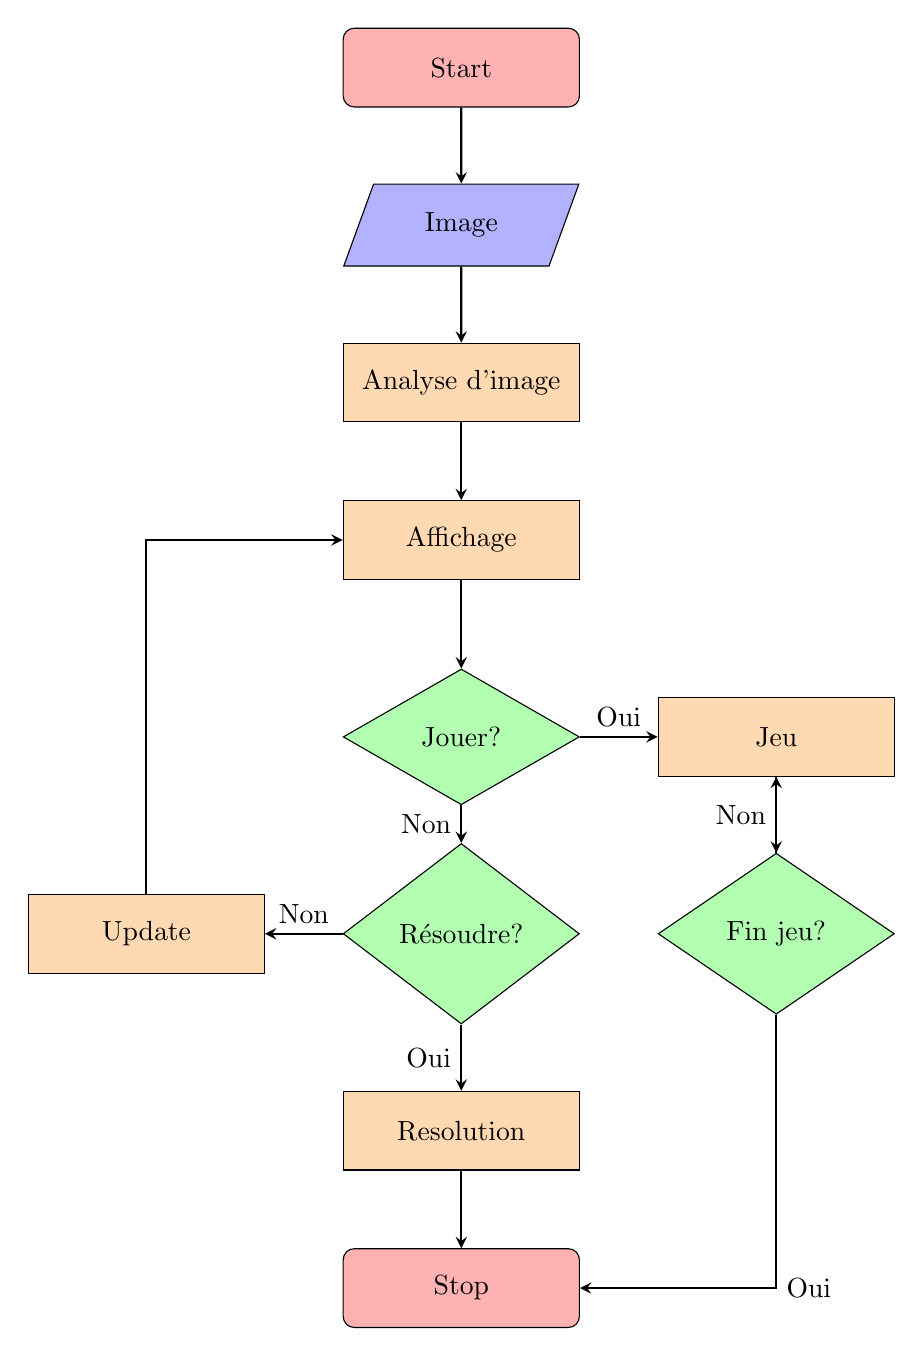
\begin{tikzpicture}[node distance=2cm]
\node (start) [startstop] {Start};
\node (in1) [io, below of=start] {Image};
\node (pro1) [process, below of=in1] {Analyse d'image};
\node (pro2) [process, below of=pro1] {Affichage};
\node (dec1) [decision, below of=pro2, yshift=-0.5cm] {Jouer?};
\node (pro2a) [process, right of=dec1, xshift=2cm] {Jeu};
\node (dec1a) [decision, below of=pro2a, yshift=-0.5cm] {Fin jeu?};
\node (dec2) [decision, below of=dec1, yshift=-0.5cm] {Résoudre?};

\node (pro3) [process, below of=dec2
, yshift=-0.5cm] {Resolution};

\node (pro4) [process, left of=dec2, xshift=-2cm] {Update};

\node (stop) [startstop, below of=pro3] {Stop};

\draw [arrow] (start) -- (in1);
\draw [arrow] (in1) -- (pro1);
\draw [arrow] (pro1) -- (pro2);
\draw [arrow] (pro2) -- (dec1);
\draw [arrow] (pro2a) -- (dec1a);
\draw [arrow] (dec1) -- node[anchor=south] {Oui}(pro2a);
\draw [arrow] (dec1a) -- node[anchor=east] {Non}(pro2a);
\draw [arrow] (dec1a) |- node[anchor=west] {Oui}(stop);
\draw [arrow] (dec1) -- node[anchor=east] {Non}(dec2);
\draw [arrow] (dec2) -- node[anchor=east] {Oui}(pro3);
\draw [arrow] (dec2) -- node[anchor=south] {Non}(pro4);

\draw [arrow] (pro4) |- (pro2);
\draw [arrow] (pro3) -- (stop);
\end{tikzpicture}

\subsection{Analyse d'image}
\subsection{Interface graphique et interaction}
\subsection{Algorithme de resolution}
\subsection{Jeu}
\subsection{Rassemblement}


\section{Implémentation du Sudoku}

\subsection{Création de l'algorithme de résolution}

La première partie consistait a créer une classe java de sudoku pour pouvoir implémenter la résolution; la solution la plus simple était de choisr une structure de données de type tableau.
\newline
\newline La deuxième étape consitait a créer des fonctions secondaires qui nous servirait pour la résolution de la grille entière; nous avons donc créer des fonctions qui testent si une valeur est absente d'un bloc, d'une colonne ou d'une ligne de la grille ; voici un exemple de l'une de ces fonctions:\\


\begin{algorithm}[H]
\SetAlgoLined
\KwData{Entier valeur,Grille grille,Entier j}
\KwResult{Renvoi vrai si la valeur n'est pas dans la colonne, faux sinon }
\For{i allant de 0 à 9}{
        \If{grille[i][j]=k}{
        \Return{Faux}
        }
        \Elf{
        \Return{Vrai}
    }
}
\caption{absentSurColonne(Entier valeur,Grille g,Entier j)}
\end{algorithm}\\\\


La troisième étape consistait à implémenter le backtrack\footnote{Aussi nommé le retour sur trace en français}.Cette fonction doit prendre une grille en entrée la résoudre et nous informer de l'état du réultat en nous renvoyant un booléen.
Il fallait donc vérifier dans la descente récursive en énumérerant tous les chiffres possibles pour observer si nous arrivions à un résultat correct ou un blocage tout cela en remplissant la grille dans la descente et si nous arrivions à un blocage nous reinitialisions la case correspondante à zéro.\\
Voici l'algorithme en question :


\begin{algorithm}[H]
\SetAlgoLined
\KwData{Grille grille,Entier position}
\KwResult{Renvoi vrai si la grille a été résolue, renvoi faux sinon}
\If{position=9*9}{\Return{Vrai} }
$i \longleftarrow position \div 9  $
$j \longleftarrow position \% 9$\\
\If{grille[i][j]!=0}{\Return{estValide(grille,postion+1);\\
\For{k allant de 1 à 9}{
\If{absentSurLigne(k,grille,i) et absentSurColonne(k,grille,j) et absentSurBloc(k,grille,i,j)}{grille[i][j] \longleftarrow k;\\
\If{estValide(grille,position+1)}{\Return{Vrai}}}
$grille[i][j] \longleftarrow 0$\\
\caption{estValide(Grille grille,Entier position)}
\Return{Faux}
}
}
}
\end{algorithm}\\

\subsection{Mise en place d'un système de reconnaissance des chiffres}
Pour réaliser le système de reconnaisance des chiffres, nous avons du utiliser la bibliothèque graphique OpenCV.
La plupart des problèmes que nous pouvons rencontrer avec cette bibliothèque ne sont très bien documentés car c'est une bibliothèque technique et utilisé surtout par des gens qualifiés.\\\\
Nous avons opté pour une implémentation permettant d'afficher sur une grille la reconnaissance d'une image provenant d'un traitement.Le but est que du moment ou l'image a été traitée elle est directement envoyé a l'IA pour qu'elle soit ensuite directement affichée sur l'application.\\

Lorsque l'utilisateur va sélectionner l'image elle sera directement envoyé au programme de traitement de l'image qui lui-même envera le résultat a l'IA qui essaiera de reconnaitre les chiffres puis d'envoyer un résultat a la classe Sudoku qui l'affichera par la suite.\\

Pour cette partie nous avons décider de nous faciliter la tâche en utilisant l'IDE eclipse car la gestion des chemins d'accès des images\footnote{En effet lors de la création d'une application Android les chemin d'accès aux images doivent provenir exclusivement du téléphone.} était plus aiséé et ainsi pouvoir observer les traitements résultants afin d'obtenir une image lisible par l'ordinateur.\\
\\

Pour implémenter ce traitement il y avait un cahier des charges à suivre :

Premièrement il fallait détecter la grille en appliquant une série de traitements à l'image a savoir:
\begin{itemize}
    \item Convertir notre image de base avec des teintes grises
    \item Appliquer un flou gaussien afin de réduire le bruit et les détails de l'image
    \item Appliquer un seuillage d'image c'est a dire convertir notre résultat précedant en noir et blanc
    \item Trouver les bordures de la grille
    \item Détecter les lignes de la grille
\end{itemize}\\

Voici ci-dessous des algorithmes de traitement de l'image utilisés par OpenCV:

Il fallait créer ensuite un système d'intelligence artificielle qui  allait essayer de comparer chaque chiffre de la grille avec des ressources et renvoyer une grille en résultat.

La derniere partie consistait a lier les trois classes c'est a dire notre classe Sudoku, celle qui manipulait l'image et l'intelligence artificielle et adapter notre code afin qu'il soit effectif sur un terminal android.

Voici ci-dessous des algorithmes de traitement de l'image utilisés par OpenCV:



\newpage
\section{Bilan et difficultés rencontrées}

\subsection{Avancement du projet}





\subsection{Difficultés rencontrées}
Pour la partie "Mise en place d'un systeme de reconnaissance de chiffres" nous avons été confrontés pour l la première fois a une bibliotheques de traitement d'image et la gestion d'une intelligence artificielle.\\\\
Nous avons donc du nous former a cette bibliothèque et après de nombreux essais nous nous ne savions pas si notre système d'IA allait réussir à détecter notre image traitée c'est pourquoi après concertation avec notre encadrant nous avons décidé d'utiliser une classe déja existante nommée ImageManipulator qui traitait l'image comme nous avions besoin afin d'être sûr que le résultat serait correct et que l'image sera ainsi facilement lisible par l'IA.Nous sommes donc parvenus a surmonter cette difficulté en utilisant des classes deja existantes a savoir une classe qui nous a permis de manipuler l'image et une classe qui nous a servi d'intelligence artificielle.\\

Ensuite malgré la grande aide que nous ont apportés ces deux classes l'adaptation du code d'eclipse à Android Studio a été très difficile car il fallait déjà réussir a installer une version d'openCV sur l'IDE Android ce qui n'a pas été chose aisée, mais aussi une fois ceci fait, trouver une version qui compilait à l'appel de la bibliothèque et vérifier qu'openCV était bien fonctionnel.\\
Ensuite plus rien ne fonctionnait de la même façon il a donc fallu créer des classes qui nous ont permis de passer outre cette difficulté et pouvoir faire l'adaptation à Android Studio.\\

Cette partie a été de loin la plus longue et la plus dure.

















\end{document}